\section{État de l'art}

\subsection{Différents types de chiffrement}

\begin{frame}
  \frametitle{\insertsubsectionhead}
  \pause
  \begin{block}{Chiffrement à différents niveaux}
    \begin{itemize}
    \item Chiffrement matériel
    \item \textbf{Chiffrement logiciel de disque}
    \item Système de fichiers chiffré
    \item Chiffrement de fichier
    \end{itemize}
  \end{block}
\end{frame}

\subsection{Chiffrement et organisation dans le système}

\begin{frame}
  \frametitle{\insertsubsectionhead}
  \pause
  \begin{block}{Chiffrement}
    \begin{itemize}
      \pause
    \item Transparent pour l'utilisateur
    \item Géré par des modules noyau
    \item Réalisé au moment de la lecture ou l'écriture
    \item Possible avec différents algorithmes
    \end{itemize}
  \end{block}
\end{frame}

\begin{frame}
  \frametitle{\insertsubsectionhead}
  \pause
  \begin{block}{Sur \textbf{Linux}}
    \begin{itemize}
      \pause
    \item Outil \textit{cryptsetup}
    \item Module \textit{dm-crypt}
    \item Standard \textit{LUKS}: \textit{Linux Ufified Key Setup}
    \item Empilement avec d'autres transformations \textit{device-mapper}
    \end{itemize}
  \end{block}
  \pause
  \begin{block}{Sur \textbf{FreeBSD}}
    \begin{itemize}
      \pause
    \item Outil et module \textit{GELI}
    \item Paramètres possibles codés en dur
    \item Empilement avec d'autres transformations \textit{GEOM}
    \end{itemize}
  \end{block}
\end{frame}

\begin{frame}
  \frametitle{\insertsubsectionhead - \textbf{Linux}}
  \begin{figure}
    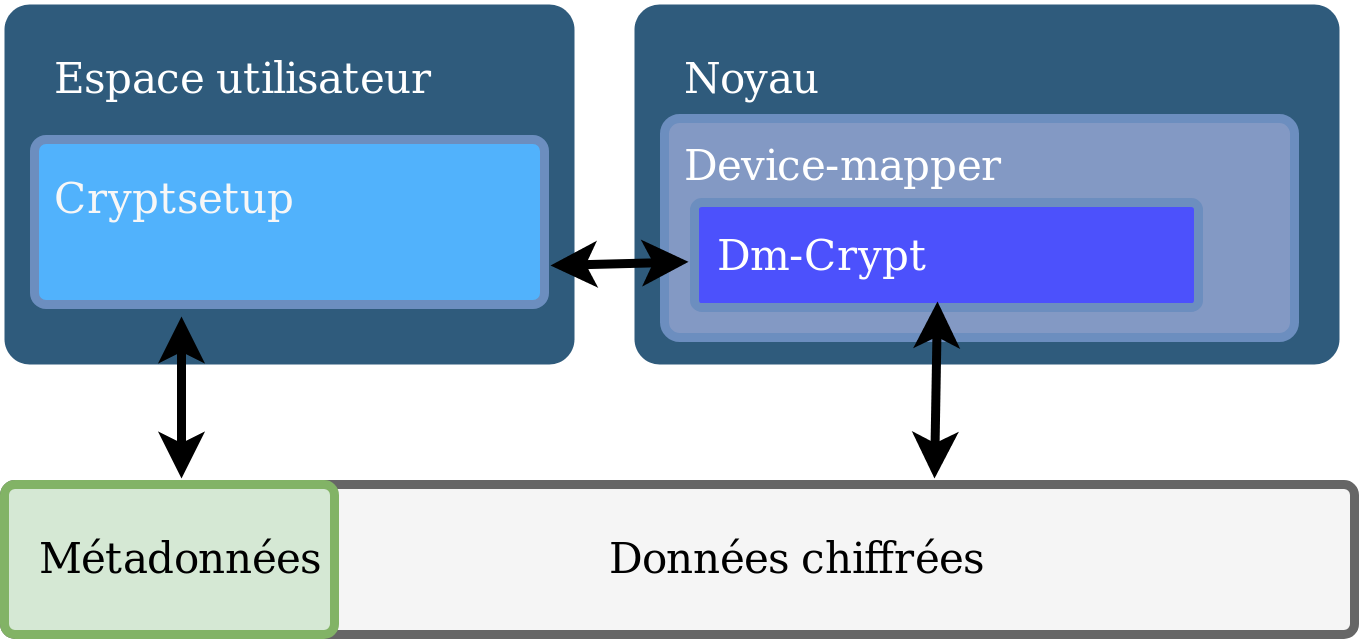
\includegraphics[width=\textwidth]{etat_art/organisation_linux}
    \caption{Organisation du code dans Linux}
  \end{figure}
\end{frame}

\begin{frame}
  \frametitle{\insertsubsectionhead - \textbf{FreeBSD}}
  \begin{figure}
    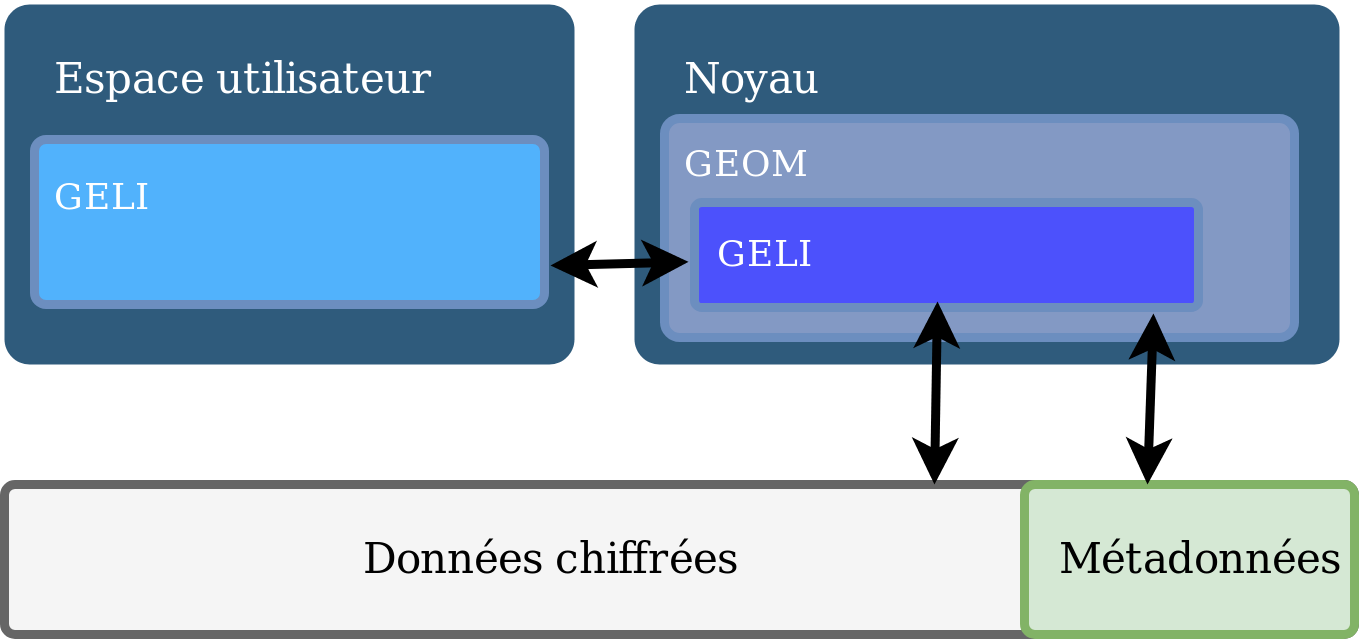
\includegraphics[width=\textwidth]{etat_art/organisation_freebsd}
    \caption{Organisation du code dans FreeBSD}
  \end{figure}
\end{frame}

\subsection{Format sur le disque}

\begin{frame}
  \frametitle{\insertsubsectionhead}
  \pause
  \begin{center}
    Format = organisation des données et métadonnées sur le disque
  \end{center}
  \pause
  \begin{block}{Format \textit{LUKS} - Linux}
    \begin{itemize}
    \item \textit{LUKS header} \textrightarrow{} métadonnées
    \item \textit{Keyslots} \textrightarrow{} 8 phrases secrètes
    \item Données chiffrées
    \end{itemize}
  \end{block}
  \pause
  \begin{block}{Format \textit{GELI} - FreeBSD}
    \begin{itemize}
    \item Données chiffrées
    \item \textit{GELI header} \textrightarrow{} métadonnées
    \end{itemize}
  \end{block}
\end{frame}

\begin{frame}
  \frametitle{\insertsubsectionhead}
  \begin{figure}
    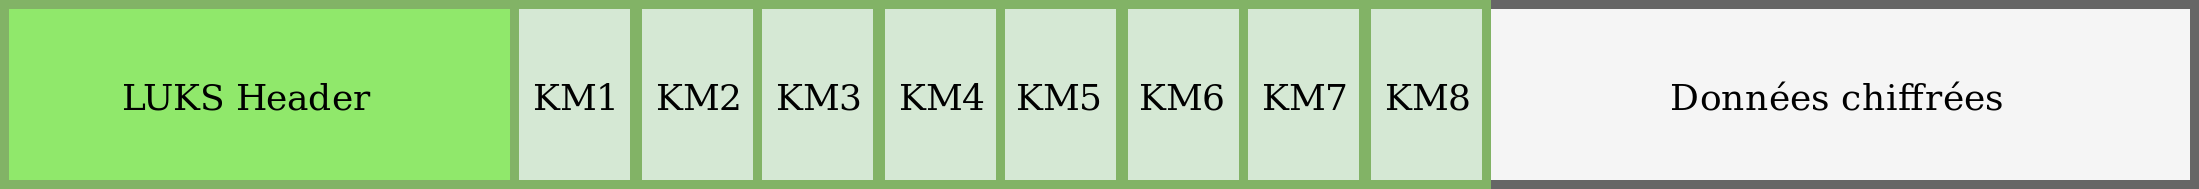
\includegraphics[width=\textwidth]{etat_art/format_disque_luks}
    \caption{Format sur disque \textit{LUKS}}
  \end{figure}
  \vfill
  \begin{figure}
    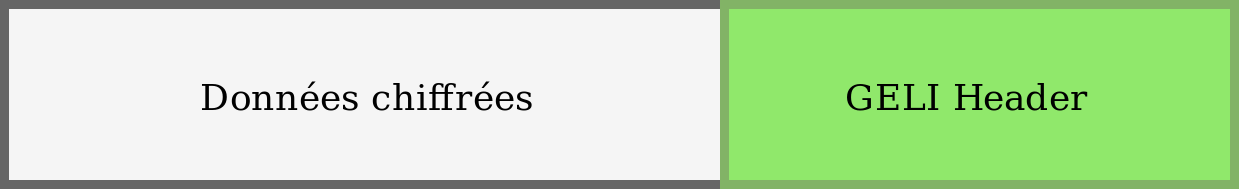
\includegraphics[width=.6\textwidth]{etat_art/format_disque_geli}
    \caption{Format sur disque \textit{GELI}}
  \end{figure}
\end{frame}

\subsection{Algorithmes communs aux deux systèmes}

\begin{frame}
  \frametitle{\insertsubsectionhead}
  \vfill
  \begin{center}
    \renewcommand{\arraystretch}{2}
    \begin{tabular}{c|*{3}{C{2cm}|}}
      \cline{2-4}
                                                     & \multicolumn{3}{c|}{\textbf{Chiffrement}}                \\ \hline
      \multicolumn{1}{|c|}{\textbf{Génération d'IV}} & \texttt{AES-XTS} & \texttt{AES-CBC} & \texttt{CAST5-CBC} \\ \hline
      \multicolumn{1}{|c|}{\texttt{plain64}}         & \textbf{X}       & \textbf{}        & \textbf{}          \\ \hline
      \multicolumn{1}{|c|}{\texttt{plain}}           & \textbf{}        & \textbf{X}       & \textbf{X}         \\ \hline
      \multicolumn{1}{|c|}{\texttt{essiv:sha256}}    & \textbf{}        & \textbf{X}       & \textbf{}          \\ \hline
    \end{tabular}
    \renewcommand{\arraystretch}{1}
  \end{center}
  \vfill
\end{frame}